\documentclass{ol-softwaremanual}

% Packages used in this example
\usepackage{graphicx}  % for including images
\usepackage{microtype} % for typographical enhancements
\usepackage{amsmath}   % for equations and mathematics
\usepackage{minted}    % for styled code blocks (requires -shell-escape + Pygments)
\usepackage{hyperref}  % for hyperlinks
\usepackage[a4paper,top=4.2cm,bottom=4.2cm,left=3.5cm,right=3.5cm]{geometry}

% Additional packages for lab content
\usepackage{enumitem}
\usepackage{changepage}  % for adjustwidth (wider code blocks)
\usepackage{tabularx}   % for width-controlled tables

% Code block style: light gray background, small monospace font, line wrapping
\setminted{style=friendly, bgcolor=gray!10, fontsize=\small, breaklines=true, breakanywhere=true}

% Wider code blocks: extend into each margin, normal text width unchanged
\newlength{\codemargin}
\setlength{\codemargin}{1.0cm}
\AddToHook{env/minted/before}{%
  \begin{adjustwidth}{-\codemargin}{-\codemargin}%
  \addtolength{\hsize}{2\codemargin}%
}
\AddToHook{env/minted/after}{\end{adjustwidth}}

% Give LaTeX extra inter-word stretch to avoid overfull boxes from long \texttt paths
\setlength{\emergencystretch}{2em}

% Machine-location badges for task headings
\newcommand{\onlaptop}{%
  \,\colorbox{green!25}{\footnotesize\sffamily\bfseries Laptop}}
\newcommand{\onrpi}{%
  \,\colorbox{blue!20}{\footnotesize\sffamily\bfseries RPi}}
\newcommand{\onui}{%
  \,\colorbox{yellow!50}{\footnotesize\sffamily\bfseries UI (browser)}}

% Machine-context callout used at the start of each Task subsection
\newcommand{\machinebox}[2]{%
  \par\noindent
  \colorbox{gray!12}{\parbox{\dimexpr\linewidth-2\fboxsep}{%
    \small\sffamily\textbf{Where to run:} #1 \quad\textbar\quad #2}}%
  \par\smallskip}

\newcommand{\doclink}[2]{\href{#1}{#2}}
\newcommand{\cs}[1]{\texttt{\textbackslash #1}}

\makeatletter
\renewcommand\maketitle{%
  \begin{titlepage}
  \centering
  \vspace*{0.18\textheight}
  \@logocmd\par
  \vspace{0.10\textheight}
  {\huge\bfseries\@title\par}
  \bigskip
  {\Large\@ver\par}
  \vfill
  {\Large\@author\par}
  \@date
  \vspace{0.06\textheight}
  \end{titlepage}
}
\makeatother

\title{Lab: Vision Node}
\version{0.1.1}
\author{162 TAs and Maclab members}
\softwarelogo{
\includegraphics[width=8cm]{figures/capstone}}

\begin{document}

\maketitle

\centerline{\textbf{Warning!}}
\begin{itemize}
    \item No food and drinks are allowed in the lab.
    \item Be careful with the hardware especially the electronics.
    \item Do not run the robot on the table — it may fall and be damaged.
    \item Be gentle to the buttons! You are liable for any damage made to the robot.
    \item Wash your hands after each experiment, some components may contain lead.
\end{itemize}
\pagebreak

\tableofcontents
\newpage


% ============================================================
\section{Overview}
% ============================================================

The \texttt{vision} ROS2 package reads frames from the Raspberry Pi camera,
runs YOLO object detection, and publishes results on the \texttt{/vision/detections}
topic.
Your robot node subscribes to this topic through the Robot API and can react to
whatever the camera sees.

\begin{figure}[h]
  \centering
  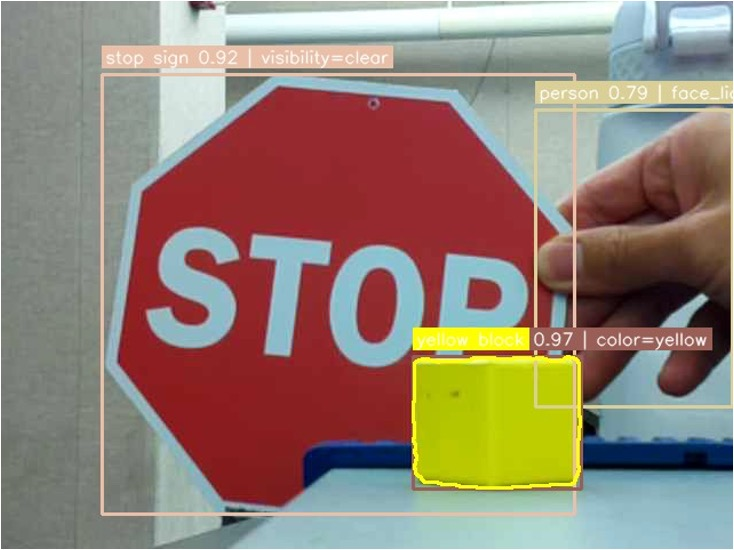
\includegraphics[width=\textwidth]{figures/detection_demo.jpg}
  \caption{Vision node output: YOLO detections overlaid on a camera frame.}
  \label{fig:detection_demo}
\end{figure}

By the end of this lab you will have completed three deliverables, each building
on the previous one:

\begin{enumerate}
  \item \textbf{Traffic light LED demo} --- The robot's onboard LEDs mirror the
        colour of a traffic light held in front of the camera.
  \item \textbf{Drive on green} --- The robot also drives forward when a green
        light is detected and stops otherwise.
  \item \textbf{(Bonus) Stop on stop sign} --- Additionally, the robot stops and
        holds whenever a stop sign is detected, regardless of the traffic light
        colour.
\end{enumerate}

\noindent\textit{Estimated time: 60 minutes for Tasks~1--4; Task~0 and Bonus Task~5 are extra.}


% ============================================================
\section{Lab Activities}
% ============================================================

% ------------------------------------------------------------
\subsection{Task 0: Update and Rebuild the Docker Image}
% ------------------------------------------------------------

\machinebox{\onrpi\ Raspberry Pi (SSH terminal)}{Only needed if your repository is not up to date. Skip this task if the TA confirms your image is current.}

If the Docker image on your Pi was built from an older version of the repository,
the vision node or bridge may be missing recent changes.
Before pulling, make sure your fork has been merged with the latest upstream
changes --- you can do this from the GitHub web interface or in the terminal.
Then pull the latest code and rebuild.

\subsubsection*{0.1 Pull Latest Changes\onrpi}

From the repository root:

\begin{minted}{bash}
git pull
\end{minted}

\subsubsection*{0.2 Rebuild the Docker Image\onrpi}

\begin{minted}{bash}
COMPOSE=ros2_ws/docker/docker-compose.rpi.yml
docker compose -f $COMPOSE build
\end{minted}

This may take several minutes on the first rebuild.

\subsubsection*{0.3 Restart the Container\onrpi}

\begin{minted}{bash}
docker compose -f $COMPOSE down
docker compose -f $COMPOSE up -d
\end{minted}

Confirm the container is running:

\begin{minted}{bash}
docker compose -f $COMPOSE ps
\end{minted}

The \texttt{ros2\_runtime} service should show \texttt{running}.


% ------------------------------------------------------------
\subsection{Task 1: Set Up the Camera Service}
% ------------------------------------------------------------

\machinebox{\onrpi\ Raspberry Pi (SSH terminal)}{One-time setup. If your team has already done this on this Pi, run only the check in step~1.2 to confirm the service is healthy.}

The Raspberry Pi CSI camera runs on the \emph{native} Ubuntu host (not inside
Docker).
A small systemd service captures frames with \texttt{rpicam-vid}, pipes them
through \texttt{ffmpeg}, and writes them into a virtual V4L2 device at
\texttt{/dev/video10}.
The Docker container reads this virtual device exactly as if it were a USB
webcam.

\subsubsection*{1.1 Install the Camera Service\onrpi}

From the repository root on the Raspberry Pi:

\begin{minted}{bash}
./ros2_ws/host_camera/install.sh
\end{minted}

The script installs \texttt{rpicam-apps}, \texttt{ffmpeg},
\texttt{v4l2loopback}, and a systemd service that starts automatically at boot.
It will prompt for \texttt{sudo} if needed.

Reboot the Pi if needed. 
\begin{minted}{bash}
sudo reboot
\end{minted}

\subsubsection*{1.2 Verify the Camera\onrpi}

\begin{minted}{bash}
./ros2_ws/host_camera/check.sh
\end{minted}

Expected final line:

\begin{minted}{text}
Results: 9 passed, 0 failed
\end{minted}

The check script saves two test images you can inspect:

\begin{minted}{text}
/tmp/pi_camera_check/host_loopback.jpg
/tmp/pi_camera_check/docker_loopback.jpg
\end{minted}

\noindent If the check fails, inspect the service log:

\begin{minted}{bash}
sudo systemctl status pi-camera-feed.service --no-pager
sudo journalctl -u pi-camera-feed.service -n 40 --no-pager
\end{minted}

A quick restart often resolves transient failures:

\begin{minted}{bash}
sudo systemctl restart pi-camera-feed.service
sleep 3
systemctl is-active pi-camera-feed.service   # should print: active
\end{minted}


% ------------------------------------------------------------
\subsection{Task 2: Verify Detections in Debug Mode}
% ------------------------------------------------------------

\machinebox{\onrpi\ Raspberry Pi (Docker shell)}{The Docker container must be running. Enter it the same way as in the previous lab.}

In debug mode the vision node saves an annotated camera frame to disk every
second.
This lets you confirm that the camera feed is working and that objects are being
detected before writing any robot code.

\subsubsection*{2.1 Open a Shell Inside the Container\onrpi}

\begin{minted}{bash}
COMPOSE=ros2_ws/docker/docker-compose.rpi.yml
docker compose -f $COMPOSE exec ros2_runtime bash
source /opt/ros/jazzy/setup.bash
source /ros2_ws/install/setup.bash
\end{minted}

\subsubsection*{2.2 Launch the Vision Node in Debug Mode\onrpi}

\begin{minted}{bash}
ros2 launch vision vision_debug.launch.py
\end{minted}

You should see log lines similar to:

\begin{minted}{text}
[vision_node]: Vision frame 640x480 total=240.3ms ncnn=228.1ms yolo=2 yellow_block=0 total=2
\end{minted}

Leave this terminal running.

\subsubsection*{2.3 View the Debug Image\onrpi}

Debug images are saved inside the container at
\texttt{/runtime\_output/vision/latest.jpg}, which is mounted to the
Raspberry Pi host at:

\begin{minted}{text}
ros2_ws/runtime_output/vision/latest.jpg
\end{minted}

Open this path in \textbf{VS Code's file browser} (via the Remote SSH
extension).
Click the file to preview it.
The image refreshes on disk every second while the vision node is running ---
click away and back, or use the VS Code refresh button, to see the latest frame.

Hold a \textbf{traffic light} or \textbf{stop sign} in front of the camera and
confirm that coloured bounding boxes appear around the detected objects.
If no detections appear, try improving the lighting or moving the object closer.

\subsubsection*{2.4 Stop the Node}

Press \textbf{Ctrl+C} in the terminal running the launch file when you are done.


% ------------------------------------------------------------
\subsection{Task 3: Traffic Light LED Demo}
% ------------------------------------------------------------

\machinebox{\onrpi\ Raspberry Pi (two Docker shells)}{You will need two terminal windows open inside the Docker container simultaneously. Open a second terminal and run the same \texttt{source} commands from Task~2.1 before continuing.}

\subsubsection*{3.1 Start the Vision Node — Terminal A\onrpi}

In the \textbf{first} Docker shell, start the vision node in production mode
(no debug image saving, lower CPU overhead):

\begin{minted}{bash}
ros2 launch vision vision_production.launch.py
\end{minted}

Keep this running throughout the rest of the lab.

\subsubsection*{3.2 Copy and Run the Example — Terminal B\onrpi}

In the \textbf{second} Docker shell, navigate to the robot package and copy the
example:

\begin{minted}{bash}
cd /ros2_ws/src/robot/robot/
cp examples/traffic_light_leds.py main.py
\end{minted}

Make sure the bridge node is running (as in previous labs), then start the robot
node:

\begin{minted}{bash}
ros2 run robot robot
\end{minted}

\subsubsection*{3.3 Test the Demo\onrpi}

Hold a red or green traffic light image (or a real light) in front of the camera:

\begin{itemize}
  \item A \textbf{green} detection → the green LED turns on.
  \item A \textbf{red} detection → the red LED turns on.
  \item No fresh detection for 2 seconds → all LEDs turn off.
\end{itemize}

\noindent When this works, you have completed \textbf{Deliverable (i)}.

\medskip\noindent\textit{Take a moment to read \texttt{traffic\_light\_leds.py}.
It is short and well-commented; Tasks~4 and~5 ask you to extend it.}


% ------------------------------------------------------------
\subsection{Task 4: Drive Forward on Green Light}
% ------------------------------------------------------------

\machinebox{\onrpi\ Raspberry Pi (Docker shell)}{Stop the robot node from Task~3 before starting. The vision node in Terminal~A should keep running.}

Extend \texttt{main.py} so the robot drives forward whenever a green light is
detected and stops otherwise.
The Robot API reference in Section~\ref{sec:robot-api} lists the methods you
will need.

Your implementation must satisfy the following requirements:

\begin{enumerate}
  \item Call \texttt{robot.set\_odometry\_parameters()} in \texttt{configure\_robot()}
        with the wheel geometry constants from \texttt{hardware\_map}
        (\texttt{WHEEL\_DIAMETER}, \texttt{WHEEL\_BASE}, \texttt{INITIAL\_THETA\_DEG},
        \texttt{LEFT\_WHEEL\_MOTOR}, \texttt{RIGHT\_WHEEL\_MOTOR}, and the
        corresponding \texttt{DIR\_INVERTED} flags).
  \item When a \textbf{green} traffic light is detected: drive forward at a
        constant speed using \texttt{robot.set\_velocity()}, and keep the green
        LED on.
  \item When a \textbf{red} traffic light is detected, or when no detection has
        arrived recently: stop the robot with \texttt{robot.stop()}.
\end{enumerate}

Run the robot node and verify:

\begin{itemize}
  \item Show a \textbf{green} light → robot drives forward, green LED on.
  \item Show a \textbf{red} light → robot stops, red LED on.
  \item Cover the camera → robot stops, LEDs off after 2 s.
\end{itemize}

\noindent When this works, you have completed \textbf{Deliverable (ii)}.


% ------------------------------------------------------------
\subsection{Task 5 (Bonus): Stop on Stop Sign}
% ------------------------------------------------------------

\machinebox{\onrpi\ Raspberry Pi (Docker shell)}{Continue editing \texttt{main.py} from Task~4.}

Add stop-sign awareness so that a stop sign overrides any traffic light command:
the robot stops and the red LED blinks whenever a stop sign is in view.

\subsubsection*{5.1 Extend the FSM\onrpi}

At the very beginning of the \texttt{elif state == "WATCHING":} block, add a
stop-sign check \emph{before} the traffic light logic:

\begin{minted}{python}
elif state == "WATCHING":
    now = time.monotonic()

    # Stop sign takes priority over traffic light colour.
    if robot.get_detections("stop sign"):
        robot.stop()
        robot.set_led(LED.RED, LED_BRIGHTNESS)
        robot.set_led(LED.GREEN, 0)
        last_shown_color = None
        lights_off_at = 0.0

    else:
        # --- existing traffic light + drive logic from Task 4 goes here ---
        traffic_light_color = find_traffic_light_color(robot)
        ...
\end{minted}

\texttt{robot.get\_detections("stop sign")} returns a list of all current
stop-sign detections.
It is non-empty whenever at least one stop sign is visible to the camera.

\subsubsection*{5.2 Test\onrpi}

\begin{itemize}
  \item Show a \textbf{green} light alone → robot drives forward.
  \item Show a \textbf{stop sign} (regardless of traffic light) → robot stops, red LED on.
  \item Remove the stop sign, show green again → robot resumes driving.
\end{itemize}

\noindent When this works, you have completed \textbf{Deliverable (iii)}.


% ============================================================
\section{Lab Deliverables}
% ============================================================

Demonstrate each deliverable to a TA in order.

\begin{enumerate}
  \item \textbf{Traffic light LED demo} --- Hold a red or green traffic light in
        front of the camera. The matching LED on the robot turns on; LEDs turn off
        when the light is removed for 2 seconds.
  \item \textbf{Drive on green} --- Show a green light: the robot drives forward.
        Show red or cover the camera: the robot stops. Demonstrate both
        transitions cleanly.
  \item \textbf{(Bonus) Stop on stop sign} --- While the robot is driving on
        green, introduce a stop sign. The robot stops immediately.
        Remove the stop sign and show green again: the robot resumes.
\end{enumerate}


% ============================================================
\section{Technical Reference}
% ============================================================

This section is optional reading. Use it when you want to go deeper or customise
the vision pipeline beyond what the tasks above cover.

\subsection{Vision Pipeline}

\begin{center}
\texttt{Pi CSI camera}
$\;\to\;$ \texttt{rpicam-vid + ffmpeg}
$\;\to\;$ \texttt{/dev/video10} (v4l2loopback)
$\;\to\;$ \texttt{vision\_node} (Docker)
$\;\to\;$ \texttt{/vision/detections} (ROS2 topic)
$\;\to\;$ \texttt{robot node}
\end{center}

Key source files inside the \texttt{vision} package:

\begin{itemize}
  \item \texttt{vision\_node.py} --- Main node: opens the camera, runs YOLO
        inference at 4~Hz, calls post-processors, and publishes detections.
  \item \texttt{model\_utils.py} --- YOLO NCNN inference wrapper and
        \texttt{DetectedObject} data class.
  \item \texttt{rule\_based\_detection.py} --- Yellow block detector (HSV colour
        thresholding, always active).
  \item \texttt{traffic\_light.py} --- Classifies a detected traffic light
        crop into \texttt{red}, \texttt{green}, or \texttt{unknown}.
  \item \texttt{stop\_sign.py} --- Classifies stop sign visibility.
  \item \texttt{launch/vision\_debug.launch.py} --- Debug mode: saves annotated
        frames to \texttt{/runtime\_output/vision/latest.jpg} at 1~Hz.
  \item \texttt{launch/vision\_production.launch.py} --- Production mode: no
        frame saving, lower CPU load.
\end{itemize}

\subsection{Detection Topic and Message Format}

The vision node publishes on the topic \texttt{/vision/detections}
using the message type
\texttt{bridge\_interfaces\allowbreak/msg\allowbreak/VisionDetectionArray}.

Each detection in the array has these fields:

\begin{center}
\begin{tabular}{lll}
\hline
\textbf{Field} & \textbf{Type} & \textbf{Meaning} \\
\hline
\texttt{class\_name} & string & Detected class, e.g.\ \texttt{"traffic light"} \\
\texttt{confidence}  & float  & Detection score, 0--1 \\
\texttt{x}, \texttt{y} & int  & Top-left corner of bounding box (pixels) \\
\texttt{width}, \texttt{height} & int & Bounding box size (pixels) \\
\texttt{attribute\_names} & string[] & Attribute labels, e.g.\ \texttt{["color"]} \\
\texttt{attribute\_values} & string[] & Attribute values, e.g.\ \texttt{["green"]} \\
\texttt{attribute\_scores} & float[]  & Confidence per attribute \\
\hline
\end{tabular}
\end{center}

\noindent You can inspect the raw topic from a Docker shell:

\begin{minted}{bash}
ros2 topic echo /vision/detections
\end{minted}

\subsection{Robot API Reference}
\label{sec:robot-api}

Call \texttt{robot.enable\_vision()} in \texttt{configure\_robot()} before using
any of the methods below.

\begin{center}
\begin{tabularx}{\linewidth}{lX}
\hline
\textbf{Method} & \textbf{What it returns / does} \\
\hline
\texttt{enable\_vision()} & Subscribe to \texttt{/vision/detections}. \\
\texttt{is\_vision\_active(t)} & \texttt{True} if a message arrived within \texttt{t} seconds. \\
\texttt{get\_detections(class\_name)} & List of detection dicts for the given class (or all if omitted). \\
\texttt{get\_detection\_attribute(cls,~attr)} & \texttt{(value, score)} for the first match, or \texttt{None}. \\
\texttt{set\_velocity(linear,~angular\_deg\_s)} & Body-frame velocity: mm/s forward, deg/s rotation. \\
\texttt{stop()} & Zero velocity on both drive wheels. \\
\hline
\end{tabularx}
\end{center}

Each detection dict returned by \texttt{get\_detections()} has the keys
\texttt{class\_name}, \texttt{confidence}, \texttt{x}, \texttt{y},
\texttt{width}, \texttt{height}, and \texttt{attributes}.
\texttt{attributes} is itself a dict mapping attribute name to
\texttt{\{"value": ..., "score": ...\}}.

\subsection{Customising the Class Filter}

By default the vision node detects \textbf{traffic lights}, \textbf{stop signs},
and \textbf{persons}.
To add or remove COCO classes, edit the \texttt{CLASSES\_OF\_INTEREST} list at
the top of \texttt{vision\_node.py}:

\begin{minted}{python}
CLASSES_OF_INTEREST = [
    "traffic light",
    "stop sign",
    "person",
    # "car",
    # "bus",
]
\end{minted}

After editing, rebuild and restart the vision node.
Valid class names are in the model metadata file:
\texttt{vision/data/yolo26n\_ncnn\_imgsz\_416/metadata.yaml}.

\subsection{Yellow Block Detection}

The vision node always runs an HSV-based yellow block detector alongside YOLO.
If you call \texttt{robot.get\_detections()} with no argument you will see
\texttt{"yellow block"} entries in the list alongside YOLO results.

Calling \texttt{robot.get\_detections("traffic light")} or any other specific
class name already filters these out --- you will not see yellow block detections
unless you explicitly ask for them.

If you want to \emph{completely} disable yellow block detection (e.g.\ to reduce
CPU load when it is not needed), comment out the yellow block call in
\texttt{vision\_node.py}:

\begin{minted}{python}
# In VisionNode.run():
yellow_block_detections, yellow_block_overlays = self._detect_yellow_block(frame)
# Comment the line above and replace with:
# yellow_block_detections, yellow_block_overlays = [], []
\end{minted}

\end{document}
